
\chapter{Arquitetura de Software}
\label{sec-arquitetura}

A arquitetura de software do sistema~\imprimirtitulo segue a arquitetura padrão sugerida pelo FrameWeb~\cite{souza:masterthesis07,souza-et-al:iism09} baseada no padrão Camada de Serviço~\cite{fowler:book02}. A Figura~\ref{figura-arquitetura-padrao} ilustra a arquitetura e indica onde atuam os \textit{frameworks} para o desenvolvimento Web, listados na Tabela~\ref{tabela-plataforma}.

\begin{figure}[h]
	\centering
	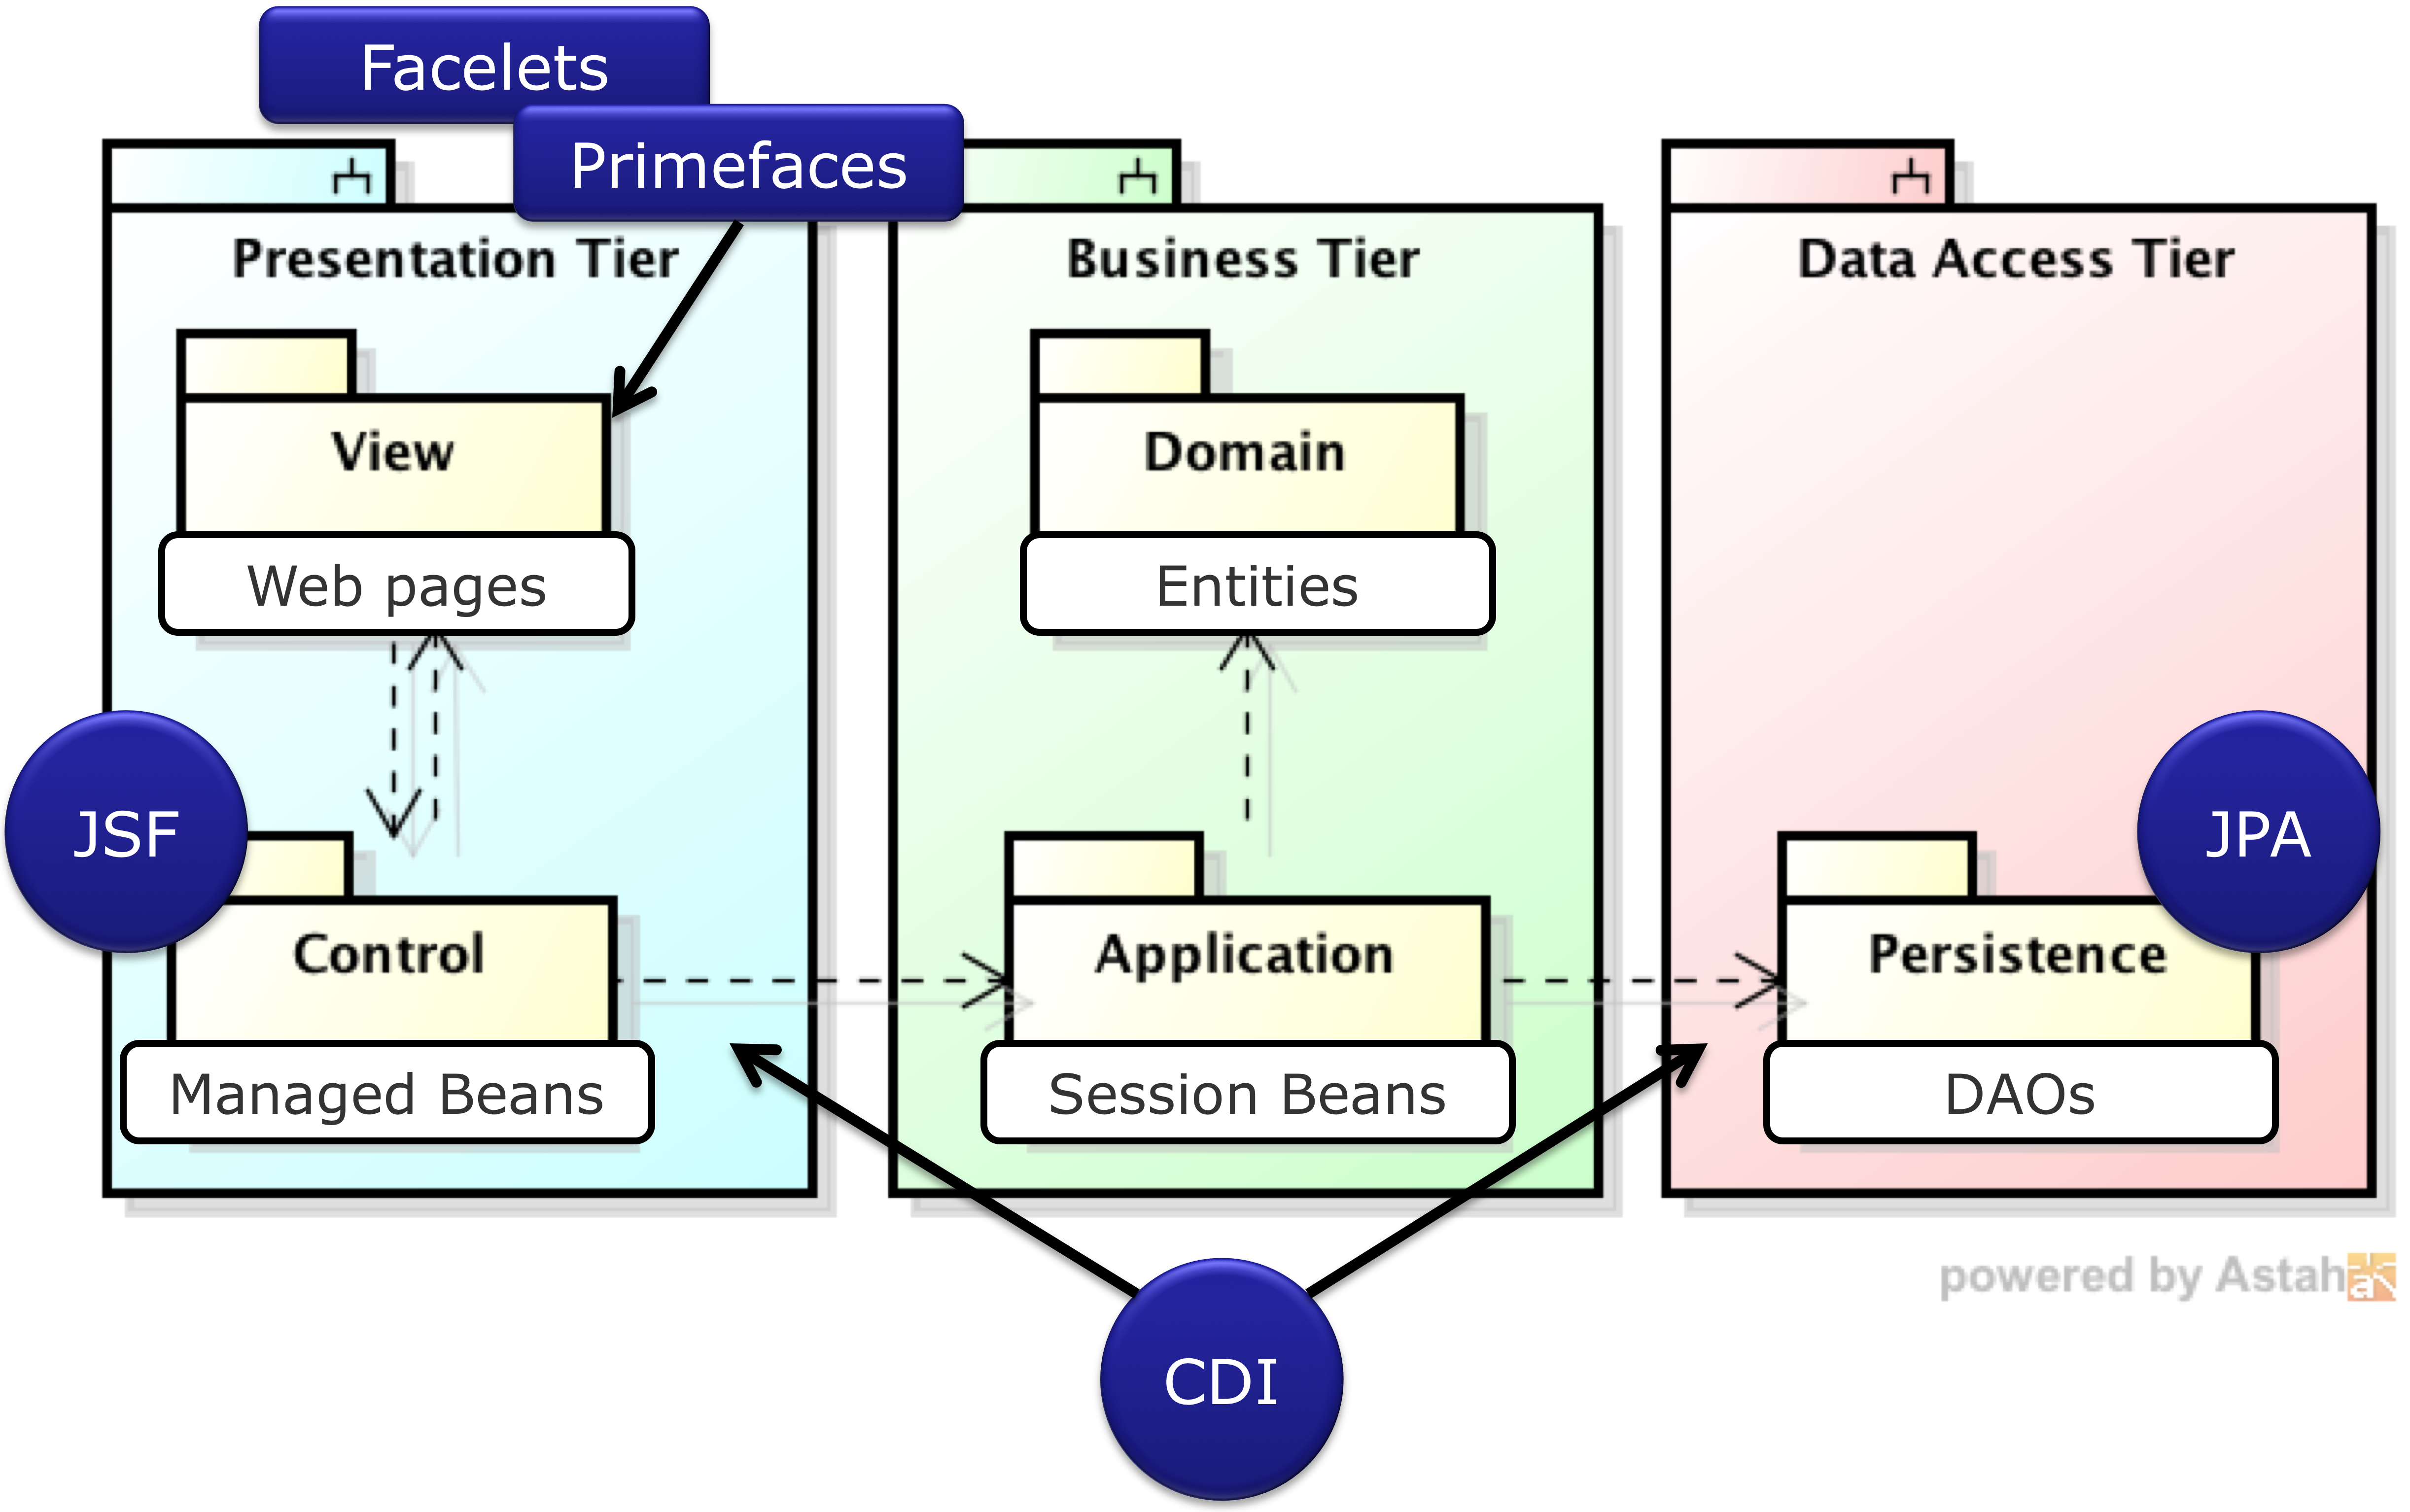
\includegraphics[width=0.8\textwidth]{figuras/figura-arquitetura-padrao.png}
	\caption{Arquitetura padrão proposta pelo FrameWeb.}
	\label{figura-arquitetura-padrao}
\end{figure}

Nas próximas seções, serão apresentados diagramas FrameWeb relativos a cada uma das camadas da arquitetura do sistema.


\section{Camada de Apresentação}
\label{sec-arquitetura-apresentacao}

\vitor{Apresentar os modelos de navegação do FrameWeb.}




\section{Camada de Negócio}
\label{sec-arquitetura-negocio}

\vitor{Apresentar os modelos de entidades e de aplicação do FrameWeb.}




\section{Camada de Acesso a Dados}
\label{sec-arquitetura-dados}

\vitor{Apresentar os modelos de persistência do FrameWeb.}

